\documentclass[10pt,conference,compsocconf]{../IEEEtran}
\usepackage{xltxtra}
\usepackage{subfig}
\usepackage{booktabs}
\usepackage{flushend}
\usepackage[numbers,sort&compress]{natbib}
\setmainfont{Times New Roman}

\begin{document}

\title{idock 1.5: Further Improving Docking Speed over idock 1.0 and AutoDock Vina}
\author
{
\IEEEauthorblockN
{
Hongjian Li, Kwong-Sak Leung and Man-Hon Wong
\IEEEauthorblockA
{
Department of Computer Science and Engineering, Chinese University of Hong Kong, Hong Kong, P.R. China\\
\{hjli, ksleung, mhwong\}@cse.cuhk.edu.hk
}
}
}
\maketitle

\begin{abstract}

In a previous study, we reported idock 1.0, a multithreaded virtual screening tool for flexible ligand docking. In this study, we report idock 1.5, further improving docking speed and accuracy, inventing new functionalities, and fixing bugs. To better evaluate and compare idock 1.5 and the state-of-the-art AutoDock Vina, we carried out a redocking benchmark on PDBbind v2011 and CSAR NRC HiQ Set 24Sept2010, and a virtual screening benchmark on 12 receptors and 3000 ligands. Results showed that under various conditions idock 1.5 displayed success rates comparable to AutoDock Vina, but outperformed AutoDock Vina in terms of docking speed by at least 8.69 and at most 37.51 times. idock is free and open source, available at https://GitHub.com/HongjianLi/idock. For future research, we are constructing a web site to provide free real-time virtual screening online, and we will port idock to the GPU using CUDA and OpenCL for further speed up. As case studies in real life, we are collaborating with biochemists and pharmacists, and utilizing idock 1.5 to discover inhibitors of influenza A virus H1N1 nucleoprotein and human cell cycle-related kinase for cancer therapy.

\end{abstract}

\section{Introduction}

Protein-ligand docking predicts the preferred conformation and binding affinity of a small ligand when it is non-covalently bound to a specific binding site of a macro protein. Up to date, there are hundreds of docking programs available. The AutoDock series is the most cited docking software in the research community. AutoDock has contributed to the discovery of several drugs, including the first clinically approved HIV integrase inhibitor \citep{1169}. Technically speaking, AutoDock is single threaded \textit{per se}. Following its initial release, several parallel implementations were developed \citep{115,560,782}, using either multithreading or computer cluster.

In 2009, AutoDock Vina \citep{595} was released. As the successor of AutoDock 4, AutoDock Vina significantly improves the average accuracy of the binding mode predictions while running two orders of magnitude faster with multithreading \citep{595}. It was compared to AutoDock 4 on selecting active compounds against HIV protease, and was recommended for docking large molecules \citep{556}. Its functionality of semi-flexible protein docking by enabling flexibility of side-chain residues was evaluated on VEGFR-2 \citep{1084}. To further facilitate the usage of AutoDock Vina, auxiliary tools were subsequently developed, including a PyMOL plugin for program settings and visualization \citep{609}, and a bootable operating system for computer clusters \citep{773}. AutoDock Vina is free and open source under Apache License 2.0. So far it has been cited by over 357 publications according to Google Scholar, making it a very competitive docking program.

In 2011, inspired by AutoDock Vina, we developed idock 1.0, a multithreaded virtual screening tool for flexible ligand docking \citep{1153}. idock inherits from AutoDock Vina the accurate scoring function and the efficient optimization algorithm, and meanwhile introduces a fruitful of innovations, such as receptor and grid map caching for large-scale virtual screening, revised numerical model for much faster approximation, capability of automatic detection and deactivation of inactive torsions, utilization of our novel thread pool to parallelize grid map creation and reuse threads, utilization of the new C++11 feature of rvalue references to avoid frequent memory reallocation, and accelerated parsers for both receptor and ligand. When benchmarked on docking 10,928 drug-like ligands against HIV reverse transcriptase, idock 1.0 achieved a speedup of 3.3 in terms of CPU time and a speedup of 7.5 in terms of elapsed time on average compared to AutoDock Vina.

Despite the amazing speedup, idock 1.0 still required about 10 hours on average to dock 10,928 drug-like ligands, not to mention massive docking of millions of ligands. Faster algorithms and implementations are highly desired. Following the release of idock 1.0 in July 2011, we then released idock 1.1 in December 2011, idock 1.2 in February 2012, idock 1.3 in March 2012, idock 1.4 in April 2012, and idock 1.5 in June 2012, further improving docking speed and accuracy, inventing new functionalities, and fixing bugs.

\section{Our Contributions to idock 1.5}

For functional improvements, idock evaluates intra-ligand free energy in addition to inter-ligand free energy, leading to lower RMSD (Root Mean Square Deviation) values between docked conformation and native conformation and thus higher prediction accuracy. idock enables automatic recovery, i.e. in case the process gets killed accidentally and restarted some time later, it not only resumes docking from the previous stopping point, skipping ligands that were already docked in a previous run, but also detects and reports possible file content errors, ensuring all the output ligands are well written. It supports as many as 29 chemical elements including rare ones like As (arsenic) and Sr (strontium), covering the majority of ligand atom types. Given a very large amount of ligands to dock, idock indirectly supports 2-phase virtual screening via two consecutive runs. In the first run, idock performs coarse but fast virtual screening without writing any conformations to file, aiming to quickly shortlist a few candidate compounds. In the second run, idock performs fine but slow virtual screening with a significantly larger number of Monte Carlo tasks per ligand, writing as many conformations to file as possible and aiming to refine the predicted free energy as well as predicted conformation of candidate compounds. Such a 2-phase docking methodology can remarkably reduce overall execution time while avoiding the risk of filtering out potentially promising compounds, controlling the false negative rate at an acceptable level.

For I/O improvements, idock supports reading and writing compressed ligand files with in gzip/bzip2 format, resulting in a file footprint as low as just one eighth of the raw size. This new functionality turns out to be extremely handy given an enormous amount of ligands to dock. idock implements our own lightweight thread-safe progress bar, reporting progress every 10\% Monte Carlo tasks per ligand. idock evaluates and outputs verbose information to docked PDBQT files, including total free energy, total inter-ligand free energy, total intra-ligand free energy, number of hydrogen bonds, and per-atom inter-ligand free energy, facilitating interaction hotspot determination and indirectly helping \textit{in silico} synthesis of potent ligands. idock writes docking summary, sorted in the ascending order of predicted free energy of docked ligands, in CSV (Comma-Separated Vector) format for subsequent analysis easily.

For computational improvements, idock better supports rvalue references and move semantics in C++11 to boost performance. idock implements our novel thread pool in order to reuse threads and maintain a high CPU utilization throughout the entire screening procedure. The thread pool parallelizes the precalculation of scoring function, the creation of grid maps, and the execution of Monte Carlo tasks. idock flattens the tree-like recursive data structure of ligand as used in AutoDock Vina into simple linear array structure to ensure a high data cache hit rate and easy coding. idock accelerates the assignment of atom types by making use of residue information for receptor and branch information for ligand. In addition to Linux and Windows, idock supports Mac OS X, FreeBSD and Solaris, making it instantly ready on the 5 mainstream operating systems.

For other miscellaneous but helpful improvements, idock allows users to specify a configuration file other than appending arguments one by one onto the command line. idock increases the number of docking examples to 12. Last the not the least, idock fixes several minor bugs. Refer to the change log for detail.

\section{Benchmarks, Results and Discussions}

idock x86\_64 v1.5 and AutoDock Vina x86 v1.1.2 were evaluated on desktop computers with Intel Core i5-2400 CPU @ 3.10GHz and 4GB DDR3 RAM under Mac OS X 10.7.4 Build 11E53. Arguments to both programs were left as default. By default, both programs output 9 predicted conformations per ligand. The benchmarks include comparison of their redocking performance in terms of predicted conformations, and comparison of their virtual screening performance in terms of execution time, memory usage, predicted free energy, and predicted conformations.

\subsection{Benchmark of Redocking Performance}

Redocking refers to randomizing the crystal ligand conformation in a protein-ligand complex and trying to dock the randomized conformation back to its crystal conformation as close as possible. For the redocking benchmark, we used two databases, PDBbind v2011 \citep{529,530} and CSAR NRC HiQ Set 24Sept2010 \citep{857,960}. The refined set of PDBbind v2011 and the two sets of CSAR NRC HiQ Set 24Sept2010 comprise 2,455 and 343 protein-ligand complexes respectively, with experimentally determined binding affinity data (Kd or Ki).

Table \ref{tab:SuccessRate} shows the success rates of idock and AutoDock Vina under various conditions regarding the RMSD values between the crystal and docked conformations. Given a redocking case, RMSD1 refers to the RMSD value between the crystal conformation and the first docked conformation, i.e. the one with the highest predicted binding affinity, while RMSDm refers to the RMSD value between the crystal conformation and the closest docked conformation, i.e. the one with the minimum RMSD value. The condition RMSD1 = RMSDm tests for how many percent the docked conformation with the highest predicted binding affinity actually turns out to be the closest one among the 9 predicted conformations. It can be seen that the success rates of idock are comparable to, albeit slightly lower than, AutoDock Vina, and the success rates on CSAR NRC HiQ Set 24Sept2010 are consistently higher than PDBbind v2011, probably because the scoring function performs well on carefully refined structures. Using a RMSD value of 2.0 \AA, a publicly accepted positive control for correct bound structure prediction, both programs manage to predict a conformation close enough to the crystal conformation as the first conformation for over half of the cases on both databases.

\begin{table}
\centering
\begin{tabular*}
{\linewidth}
{@{\extracolsep{\fill}}crrrr}
\toprule
& \multicolumn{2}{c}{PDBbind v2011} & \multicolumn{2}{c}{CSAR NRC HiQ}\\
Condition & idock & Vina & idock & Vina\\
\midrule
RMSD1 = RMSDm   & 47\% & 54\% & 57\% & 71\%\\
RMSD2 = RMSDm   & 16\% & 14\% & 17\% & 13\%\\
RMSD3 = RMSDm   &  8\% &  8\% &  7\% &  4\%\\
RMSD4 = RMSDm   &  6\% &  5\% &  5\% &  3\%\\
RMSD5 = RMSDm   &  5\% &  5\% &  4\% &  1\%\\
RMSD6 = RMSDm   &  5\% &  4\% &  3\% &  3\%\\
RMSD7 = RMSDm   &  5\% &  4\% &  1\% &  2\%\\
RMSD8 = RMSDm   &  4\% &  3\% &  3\% &  2\%\\
RMSD9 = RMSDm   &  4\% &  3\% &  3\% &  2\%\\
RMSD1 < 0.5 \AA & 11\% & 12\% & 21\% & 21\%\\
RMSD1 < 1.0 \AA & 29\% & 31\% & 40\% & 47\%\\
RMSD1 < 1.5 \AA & 45\% & 47\% & 61\% & 67\%\\
RMSD1 < 2.0 \AA & 53\% & 56\% & 68\% & 73\%\\
RMSDm < 0.5 \AA & 14\% & 15\% & 24\% & 26\%\\
RMSDm < 1.0 \AA & 39\% & 40\% & 54\% & 55\%\\
RMSDm < 1.5 \AA & 64\% & 65\% & 78\% & 84\%\\
RMSDm < 2.0 \AA & 74\% & 78\% & 86\% & 92\%\\
\bottomrule
\end{tabular*}
\caption{Success rates of idock and AutoDock Vina under various conditions on PDBbind v2011 and CSAR NRC HiQ Set 24Sept2010.}
\label{tab:SuccessRate}
\end{table}

Figure \ref{fig:FECorrelation} shows the free energy correlation of idock and AutoDock Vina. On the CSAR NRC HiQ Set 24Sept2010 database, the Pearson correlations between experimental binding affinity and free energy predicted by AutoDock Vina, between experimental binding affinity and free energy predicted by idock, and between free energy predicted by AutoDock Vina and idock are -0.5998758, -0.5774972, and 0.9824049, respectively. The experimental binding affinity is positive while the predicted free energy is negative, hence the negative sign for the former two correlations. It can be seen that both programs fail to predict reliable free energy, a very common obstacle in the entire research community. As expected, the correlation between free energy predicted by both programs is very close to 1 because of their identical scoring function.

\begin{figure*}
\centering
\subfloat[PDBbind v2011]
{
  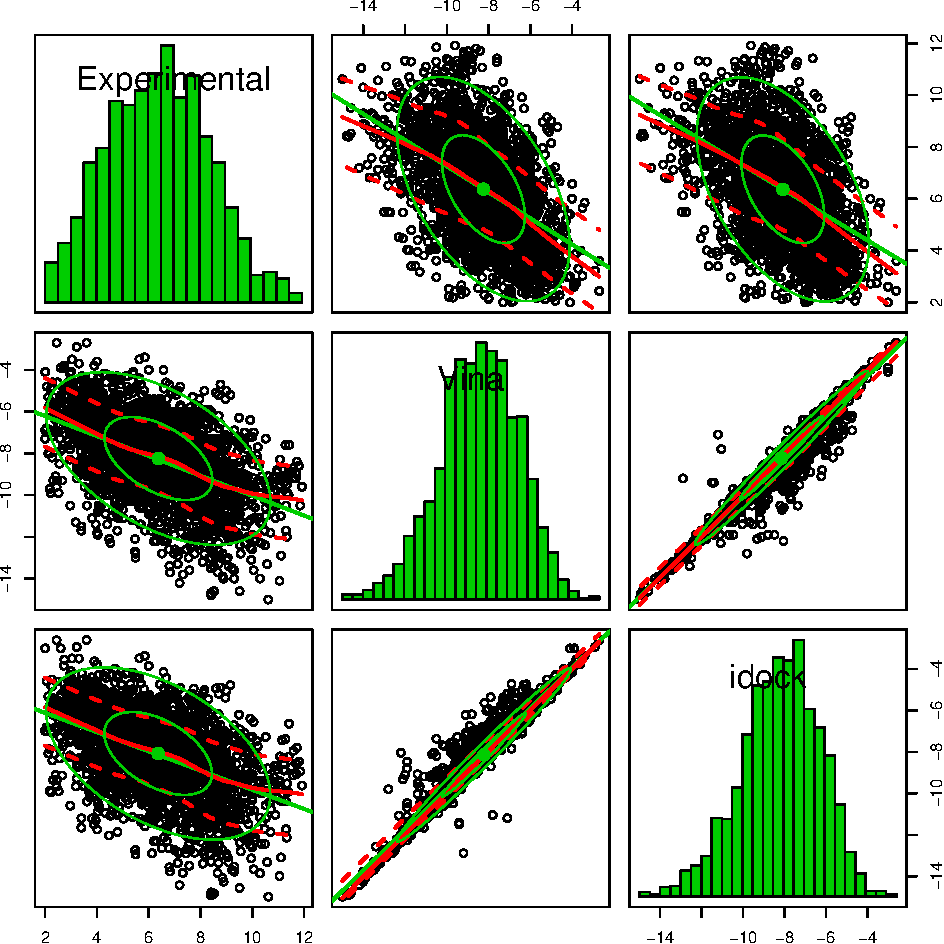
\includegraphics[width=0.485\linewidth]{PDBbindFECorrelation.pdf}
}
\subfloat[CSAR NRC HiQ Set 24Sept2010]
{
  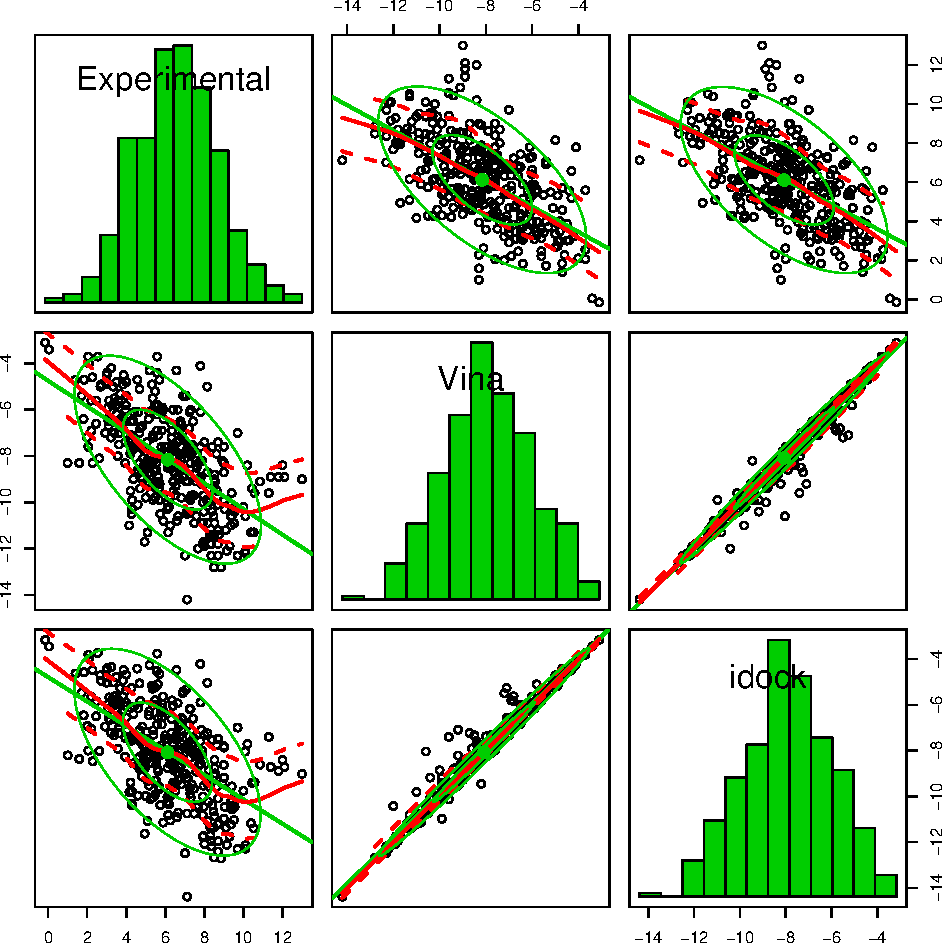
\includegraphics[width=0.485\linewidth]{CSARFECorrelation.pdf}
}
\caption{Free energy correlation on PDBbind v2011 and CSAR NRC HiQ Set 24Sept2010.}
\label{fig:FECorrelation}
\end{figure*}

\subsection{Benchmark of Virtual Screening Performance}

We collected 12 receptors from the PDB (Protein Data Bank) database \cite{540,537}, and 1000 ligands with a molecular weight of 200-300g/mol2, 1000 ligands with a molecular weight of 300-400g/mol2, and 1000 ligands with a molecular weight of 400-500g/mol2 from the clean subset of the ZINC database \cite{532,1178}. The 3000 ligands (Figure \ref{fig:MWT-NRB}) were docked against the 12 receptors by Vina and idock. Since Vina can dock only one ligand in each run, a bash script containing 1000 lines was executed instead, with each line being an execution of Vina to dock one individual ligand. The GNU Time utility was used as profiler.

\begin{figure*}
\centering
\subfloat
{
  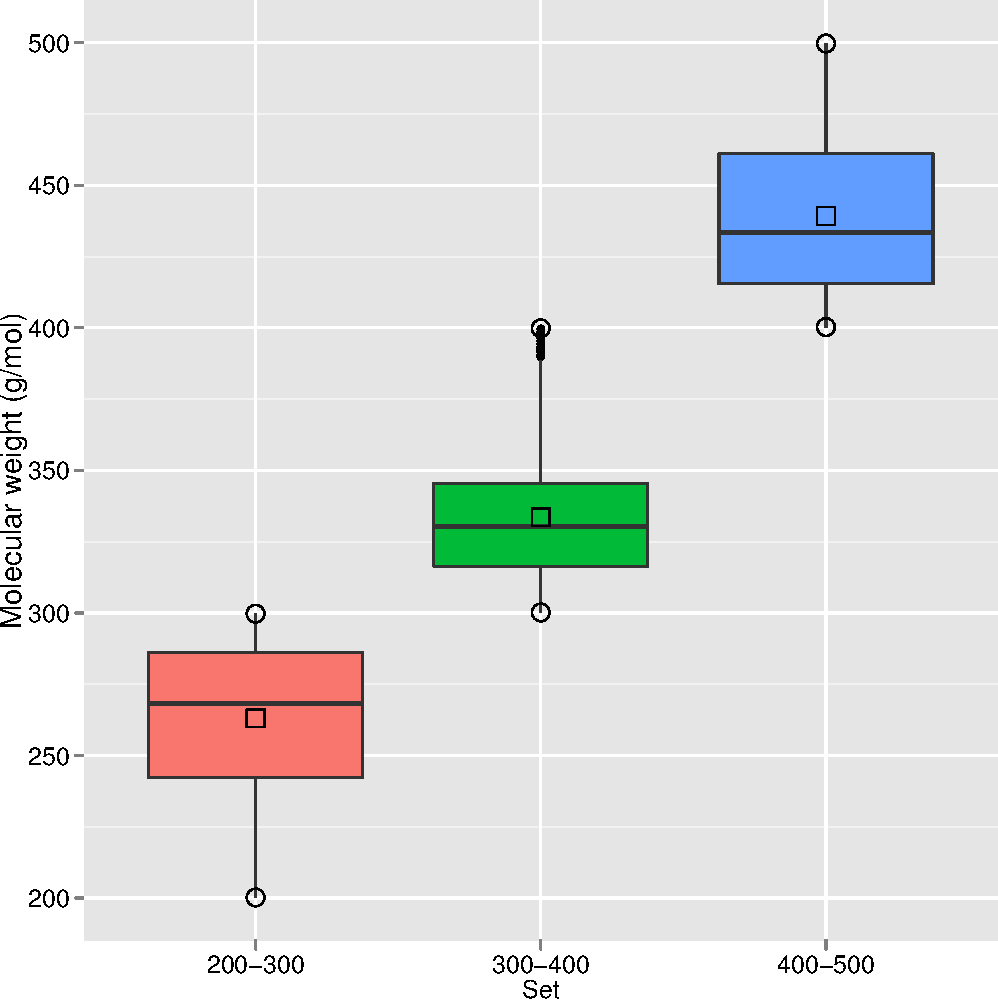
\includegraphics[width=0.485\linewidth]{MWT.pdf}
}
\subfloat
{
  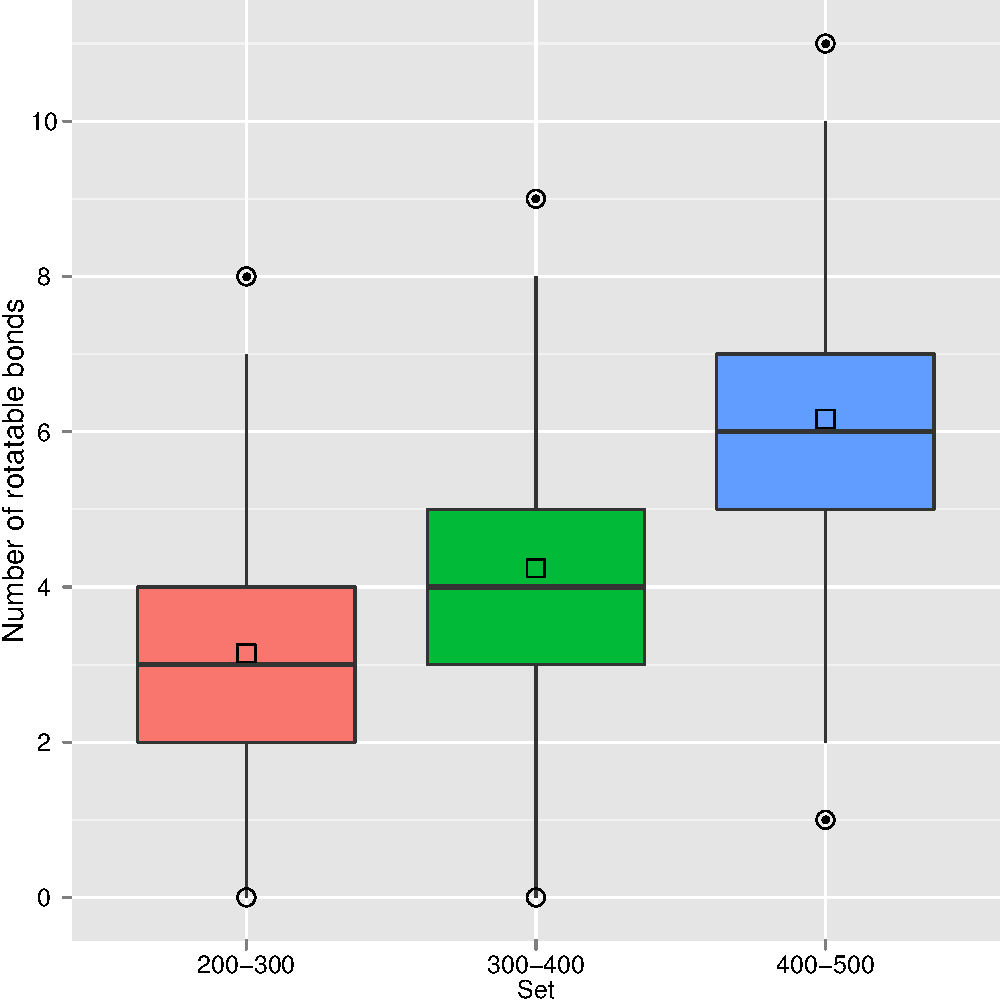
\includegraphics[width=0.485\linewidth]{NRB.pdf}
}
\caption{Boxplot of molecular weight and number of rotatable bonds of ligands of the three molecular weight sets.}
\label{fig:MWT-NRB}
\end{figure*}

Table \ref{tab:ExecutionTime} compares the CPU time and elapsed time of both programs. The execution time varies a lot from receptor to receptor and from molecular weight set to set, so does the ratio. Basically idock outperforms Vina by at least 8.69 and at most 37.51.

\begin{table}
\centering
\begin{tabular*}
{\linewidth}
{@{\extracolsep{\fill}}crrrrrr}
\toprule
& \multicolumn{2}{c}{200-300g/mol} & \multicolumn{2}{c}{300-400g/mol} & \multicolumn{2}{c}{400-500g/mol}\\
Program & CPU & Elapsed & CPU & Elapsed & CPU & Elapsed\\
\midrule
\multicolumn{7}{l}{\textbf{1HCL} human cyclin-dependent kinase 2}\\
Vina  & 12.57 &  3.33 & 22.55 &  5.91 & 51.62 & 13.41\\
idock &  0.63 &  0.16 &  0.92 &  0.24 &  1.38 &  0.36\\
Ratio & 20.06 & 20.25 & 24.41 & 24.39 & 37.51 & 36.81\\
\noalign{\smallskip\smallskip}
\multicolumn{7}{l}{\textbf{1J1B} human tau protein kinase I}\\
Vina  &  9.07 &  2.47 & 14.69 &  3.92 & 32.28 &  8.49\\
idock &  0.78 &  0.21 &  1.25 &  0.33 &  2.35 &  0.62\\
Ratio & 11.55 & 11.92 & 11.73 & 11.87 & 13.73 & 13.73\\
\noalign{\smallskip\smallskip}
\multicolumn{7}{l}{\textbf{1LI4} human S-adenosylhomocysteine hydrolase}\\
Vina  & 11.82 &  3.30 & 19.08 &  5.22 & 39.41 & 10.64\\
idock &  0.89 &  0.23 &  1.55 &  0.40 &  3.15 &  0.82\\
Ratio & 13.24 & 14.14 & 12.33 & 12.95 & 12.50 & 12.98\\
\noalign{\smallskip\smallskip}
\multicolumn{7}{l}{\textbf{1V9U} human rhinovirus 2 coat protein VP1}\\
Vina  &  9.80 &  2.95 & 15.55 &  4.62 & 29.75 &  8.49\\
idock &  0.97 &  0.25 &  1.64 &  0.42 &  3.42 &  0.89\\
Ratio & 10.11 & 11.74 &  9.49 & 10.91 &  8.69 &  9.56\\
\noalign{\smallskip\smallskip}
\multicolumn{7}{l}{\textbf{2IQH} influenza A virus nucleoprotein NP}\\
Vina  &  9.51 &  2.66 & 15.03 &  4.08 & 29.64 &  7.83\\
idock &  0.92 &  0.24 &  1.59 &  0.41 &  3.41 &  0.88\\
Ratio & 10.35 & 11.18 &  9.43 &  9.93 &  8.69 &  8.93\\
\noalign{\smallskip\smallskip}
\multicolumn{7}{l}{\textbf{2XSK} Escherichia coli curli protein CsgC - SeCys}\\
Vina  & 10.44 &  2.71 & 17.89 &  4.61 & 40.58 & 10.41\\
idock &  0.71 &  0.19 &  1.16 &  0.30 &  2.16 &  0.56\\
Ratio & 14.68 & 14.64 & 15.47 & 15.38 & 18.83 & 18.57\\
\noalign{\smallskip\smallskip}
\multicolumn{7}{l}{\textbf{2ZD1} HIV-1 reverse transcriptase}\\
Vina  &  9.78 &  2.70 & 17.67 &  4.76 & 42.03 & 11.33\\
idock &  0.97 &  0.25 &  1.52 &  0.39 &  2.60 &  0.69\\
Ratio & 10.05 & 10.73 & 11.61 & 12.07 & 16.14 & 16.54\\
\noalign{\smallskip\smallskip}
\multicolumn{7}{l}{\textbf{2ZNL} influenza virus RNA polymerase subunit PA}\\
Vina  &  9.49 &  2.60 & 15.04 &  4.01 & 29.97 &  7.82\\
idock &  0.89 &  0.23 &  1.56 &  0.40 &  3.41 &  0.87\\
Ratio & 10.70 & 11.37 &  9.65 & 10.06 &  8.78 &  8.98\\
\noalign{\smallskip\smallskip}
\multicolumn{7}{l}{\textbf{3BGS} human purine nucleoside phosphorylase}\\
Vina  &  9.59 &  2.57 & 16.50 &  4.37 & 38.42 & 10.14\\
idock &  0.95 &  0.25 &  1.55 &  0.40 &  2.81 &  0.74\\
Ratio & 10.09 & 10.45 & 10.65 & 10.89 & 13.65 & 13.75\\
\noalign{\smallskip\smallskip}
\multicolumn{7}{l}{\textbf{3H0W} human S-adenosylmethionine decarboxylase}\\
Vina  &  9.85 &  2.64 & 17.67 &  4.70 & 41.69 & 11.04\\
idock &  0.88 &  0.23 &  1.35 &  0.35 &  2.20 &  0.58\\
Ratio & 11.17 & 11.50 & 13.07 & 13.28 & 18.99 & 19.11\\
\noalign{\smallskip\smallskip}
\multicolumn{7}{l}{\textbf{3IAR} human adenosine deaminase}\\
Vina  & 11.25 &  3.03 & 20.21 &  5.39 & 46.93 & 12.53\\
idock &  0.80 &  0.21 &  1.21 &  0.32 &  2.01 &  0.53\\
Ratio & 14.10 & 14.44 & 16.68 & 16.90 & 23.34 & 23.59\\
\noalign{\smallskip\smallskip}
\multicolumn{7}{l}{\textbf{3KFN} HIV protease}\\
Vina  & 10.53 &  2.80 & 18.37 &  4.83 & 42.43 & 11.03\\
idock &  0.77 &  0.20 &  1.20 &  0.32 &  2.09 &  0.55\\
Ratio & 13.69 & 13.85 & 15.29 & 15.32 & 20.32 & 20.12\\
\noalign{\smallskip\smallskip}
\multicolumn{7}{l}{\textbf{Average across the above 12 receptors}}\\
Vina  & 10.31 &  2.81 & 17.52 &  4.70 & 38.73 & 10.26\\
idock &  0.85 &  0.22 &  1.38 &  0.36 &  2.58 &  0.67\\
Ratio & 12.48 & 13.02 & 13.32 & 13.66 & 16.76 & 16.89\\
\bottomrule
\end{tabular*}
\caption{CPU time and elapsed time in hours of docking 3000 clean ligands of 3 molecular weight sets against 12 receptors by Vina and idock.}
\label{tab:ExecutionTime}
\end{table}

\section{Availability}

idock is free and open source under Apache License 2.0. Precompiled executables for 32-bit and 64-bit Linux, Windows, Mac OS X, FreeBSD and Solaris, 12 docking examples, and a doxygen file for generating API documentations are available at https://github.com/HongjianLi/idock.

\section{Future Directions}

We are actively developing istar, a SaaS (Software as a Service) platform for idock. The goal of istar is to automate virtual screening. Without tedious software installation, users, especially computational chemists, can submit docking jobs on the fly in either of three ways: browsing our web site, programming against our RESTful API, or sending emails conforming to our specifications. Upon job completion, users can download top hits and seek for purchasing information.

At the same time, we will port idock to the GPU using CUDA and OpenCL, aiming at further speeding up idock by at least an order of magnitude. We will also incorporate click chemistry into idock for \textit{in silico} synthesis of novel ligands.

\section{Real-Life Drug Discovery Case Studies}

Our colleagues and collaborators as biochemists and pharmacists are working on several high-impact drug discovery projects. They have done lots of biological assays and succeeded in identifying pharmaceutical and druggable protein targets for certain diseases. They outsource the docking tasks to us, hoping to discover potent and selective inhibitors of certain proteins.

\subsection{Influenza A Virus H1N1}

Prof. Pang-Chui Shaw and his team from Department of Biochemistry at Chinese University of Hong Kong have studied influenza A virus H1N1 (swine flu) for years. They select the influenza viral nucleoprotein as drug target, and we assist with structure-based virtual screening.

The influenza viral nucleoprotein forms the protein scaffold of the helical genomic ribonucleoprotein complexes, and interacts with the viral RNA polymerase to promote viral RNA replication. Oligomerization of the nucleoprotein is mediated by a flexible tail loop that is inserted into the body domain of a neighbouring molecule and makes extensive interactions through intermolecular $\beta$-sheets, hydrophobic interactions and salt bridges \citep{1140} (Figure \ref{Case:InfluenzaNucleoprotein}, reprinted from \citep{1140}). The displacement of the tail loop from its binding pocket causes significant structural rearrangements in nucleoprotein. Chemical compounds which competitively displace the tail loop from its binding pocket would interfere with viral genome replication, and therefore serve as promising leads for anti-influenza drug development \citep{1140}.

\begin{figure}
\centering
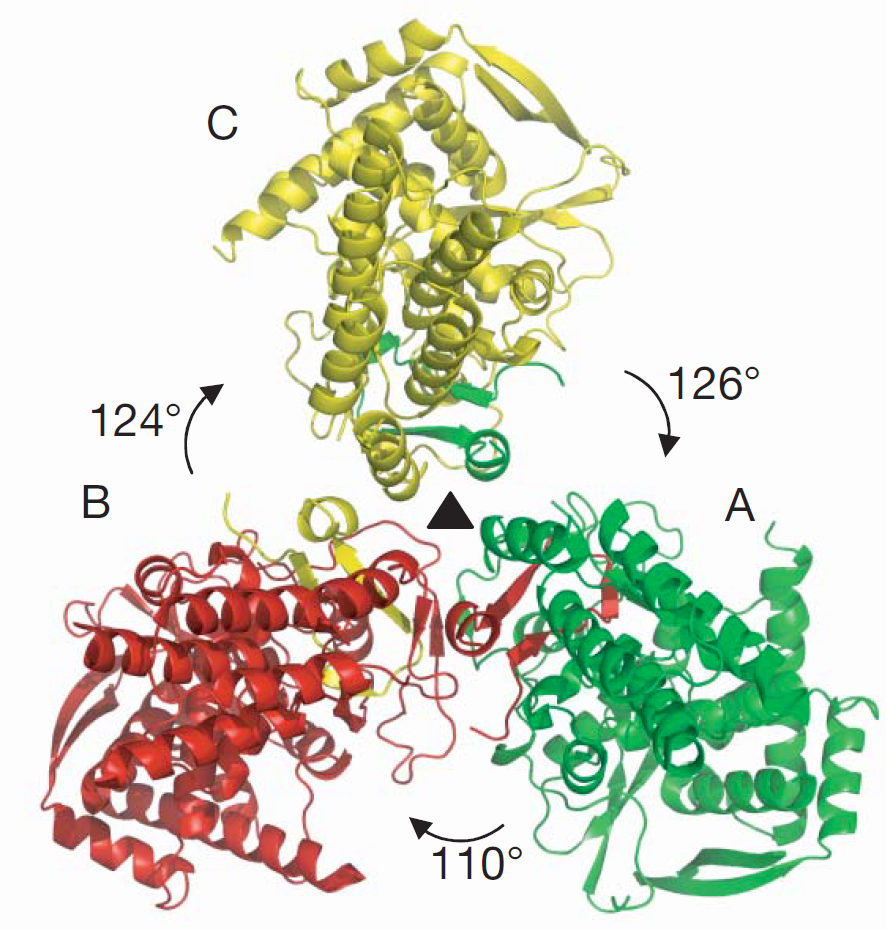
\includegraphics[width=\linewidth]{Case/InfluenzaNucleoprotein.png}
\caption{Nucleoprotein trimer viewed along the NCS (Non-Crystallographic Symmetry) three-fold axis, with three subunits shown in different colours. The rotation angles that relate the three subunits are marked. Figure reprinted from \citep{1140}.}
\label{Case:InfluenzaNucleoprotein}
\end{figure}

We are collaborating with Prof. Shaw's team on identifying inhibitors of influenza A H1N1. We obtained the X-ray crystal structures of influenza viral nucleoprotein with PDB ID 2IQH \citep{1140} and influenza A RNA polymerase subunits PA-PB1 complex with PDB ID 2ZNL \citep{1141}. For the nucleoprotein, we removed chains B and C and only retained chain A. For the PA-PB1 complex, we removed PB1 and only retained PA. Using idock 1.4 with a fine grid map granularity of 0.08\AA, we started virtual screening 7,220,835 ZINC \citep{532,1178} clean ligands whose molecular weight is above 350g/mol against the nucleoprotein chain A. The 7 million ligands are organized into 98 slices, with 34 slices currently done. Such a 35\% progress took us 1.5 months. Figure \ref{Case:2IQHHits} depicts the interactions between influenza viral nucleoprotein chain A and two high-rank ligands. Such precious experience builds us strong confidence to subsequently work on other influenza A subtypes like H5N1 (bird flu).

\begin{figure*}
\centering
\subfloat[Influenza viral nucleoprotein chain A in complex of ZINC20464531, which forms 4 hydrogen bonds with VAL186, GLY268 and HIS272, Pi-Pi interactions with TRP330, and Pi-Cation interaction with HIS272 and ARG389.]
{
  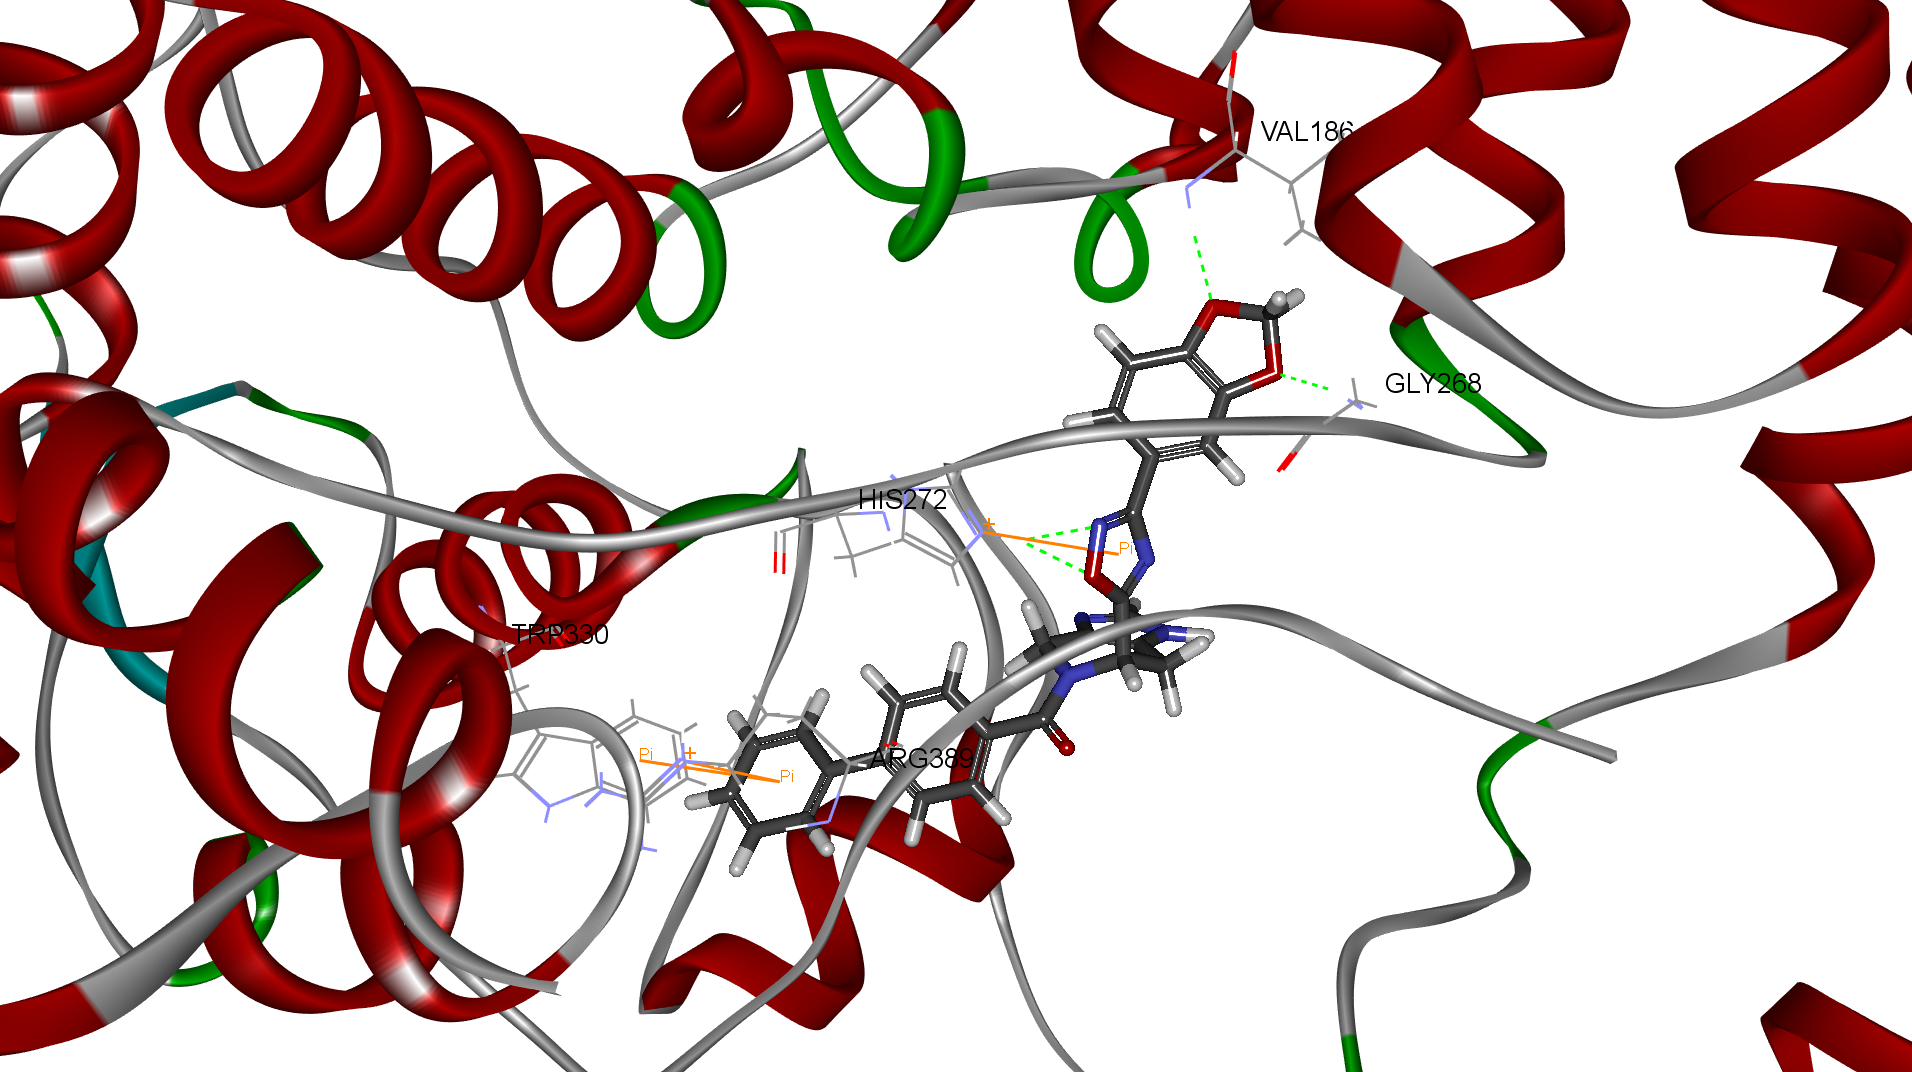
\includegraphics[width=0.485\linewidth]{Case/2IQH-ZINC20464531.png}
}
\subfloat[Influenza viral nucleoprotein chain A in complex with ZINC33733935, which forms 3 hydrogen bonds with HIS272 and THR390, Pi-Pi interactions with PHE458, and Pi-Cation interaction with ARG267.]
{
  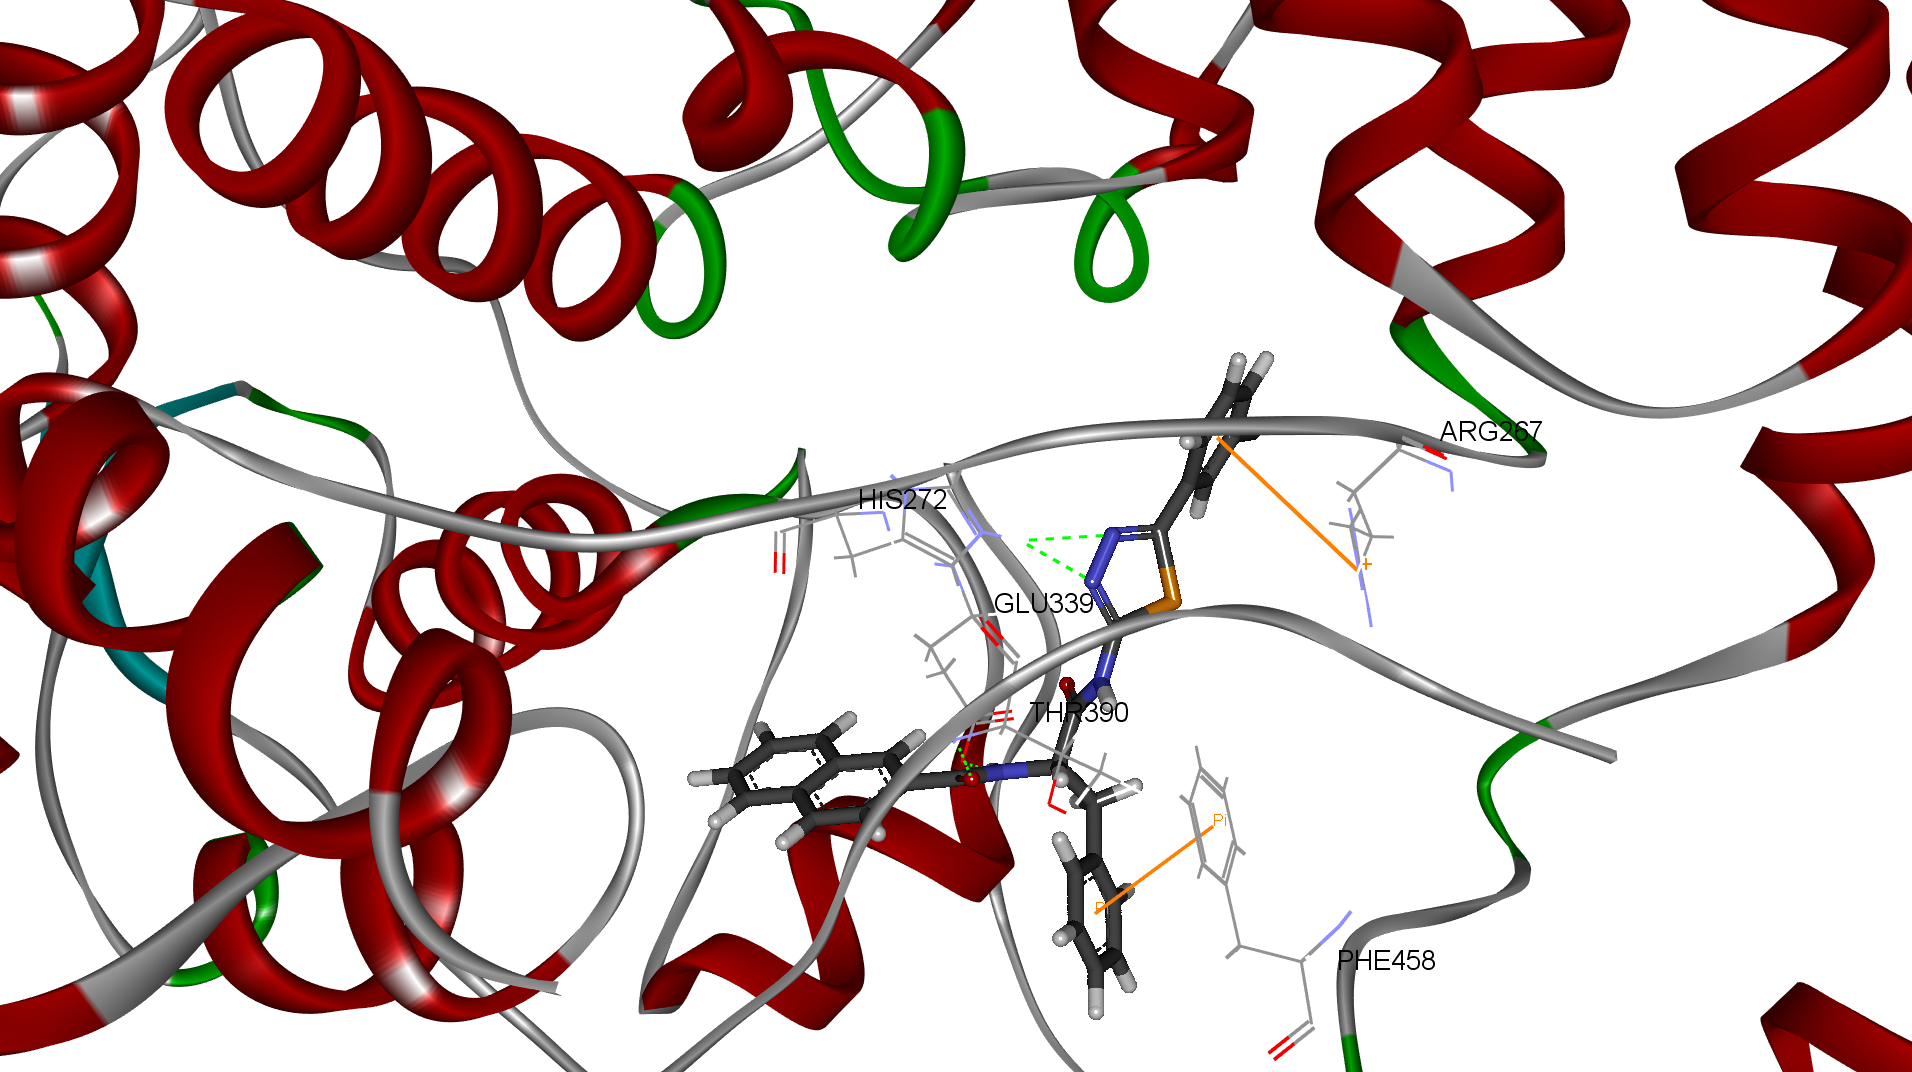
\includegraphics[width=0.485\linewidth]{Case/2IQH-ZINC33733935.png}
}
\caption{Two high-rank ligands for influenza viral nucleoprotein.}
\label{Case:2IQHHits}
\end{figure*}

\subsection{Tumors and Carcinomas}

Prof. Marie Chia-Mi Lin and her team from Department of Surgery at Prince of Wales Hospital together with the team at the State Key Laboratory of Oncology in Southern China at Sun Yat-Sen University investigated the involvement of CCRK (Cell Cycle-Related Kinase) in glioblastoma multiforme carcinogenesis. They analyzed the expression levels of CCRK in 26 glioma patient samples and normal brain, and observed that 1) knock down of CCRK by siRNA (small-interfering RNA) inhibited glioblastoma cell proliferation, 2) suppression of CCRK by shRNA (short hairpin RNA) inhibited glioblastoma tumor growth in nude mice, and 3) CCRK overexpression conferred tumorigenicity to a non-tumorigenic U-138 cell line, and concluded CCRK to be a candidate oncogene in glioblastoma multiforme tumorigenesis \citep{1144}.

Moreover, they examined CCRK expression in a series of ovarian carcinoma tissues by immunohistochemistry, and detected overexpression of CCRK in 53\% of the ovarian carcinomas, and found it positively correlated with patients' clinicopathological characteristics \citep{1145}. They also investigated the role of CCRK in human colorectal cancer carcinogenesis, and found that CCRK protein levels were elevated by more than 1.5-fold in 70\% of colorectal cancer patient samples examined and CCRK was detectable in all seven colorectal cancer cell lines tested \citep{1143}. Suppression of CCRK by siCCRK led to G1 phase cell cycle arrest and reduced cell growth. CCRK is required for the phosphorylation of CDK2 (Cyclin-Dependent Kinase 2) on Thr160 and Rb on Ser795 and the expression of cyclin E \citep{1143}. 

Furthermore, together with Prof. Joseph Jao-Yiu Sung's team, they used genome-wide location and functional analyses to identify CCRK as a direct androgen receptor-regulated gene that drives $\beta$-catenin/T cell factor-dependent hepatocarcinogenesis \citep{1146}. Conversely, knock down of CCRK decreased hepatocellular carcinoma cell growth. CCRK overexpression correlated with the tumor staging and poor overall survival of patients \citep{1146}.

They therefore attempted to seek for CCRK inhibitors for the treatment of cancers and drug resistances. Due to the absence of CCRK structure in the PDB database \citep{540,537}, they utilized Chem3D from the then CambridgeSoft company, now acquired by PerkinElmer, Inc., to build a homologous model of CCRK from CDK2 based on the fact that they share 35\% sequence identity, and performed protein-ligand docking of TCMs (Traditional Chinese Medicines) with AutoDock 3.0.5 and Cerius2 LigandFit, and identified 22-O-Angeloyl theasapogenol B as a potential potent inhibitor that could fit into the deep and narrow active site of their homologous model of CCRK. It was, nevertheless, very difficult to purify the compound from puerh tea.

We are collaborating with Prof. Lin's team on identifying inhibitors of CCRK. We used as receptor the CCRK homologous model (Figure \ref{Case:CCRKHomologousModel}) built by Dr. William Cheung based on the CDK2 template with PDB ID 1HCL \citep{1142} using SWISS-MODEL, a fully automated protein structure homology-modeling server accessible via the ExPASy web server. We concentrated on repurposing approved drugs because they display preferable ADMET properties and thus save us from dispensable clinical trials. Using idock 1.5 with a fine grid map granularity of 0.08\AA\ and 512 Monte Carlo tasks, we screened 1,715 FDA-approved drugs via DrugBank and 3,176 FDA-approved drugs via DSSTOX. Figure \ref{Case:1HCLHits} depicts the interactions between the CCRK homologous model and two high-rank ligands.

\begin{figure}
\centering
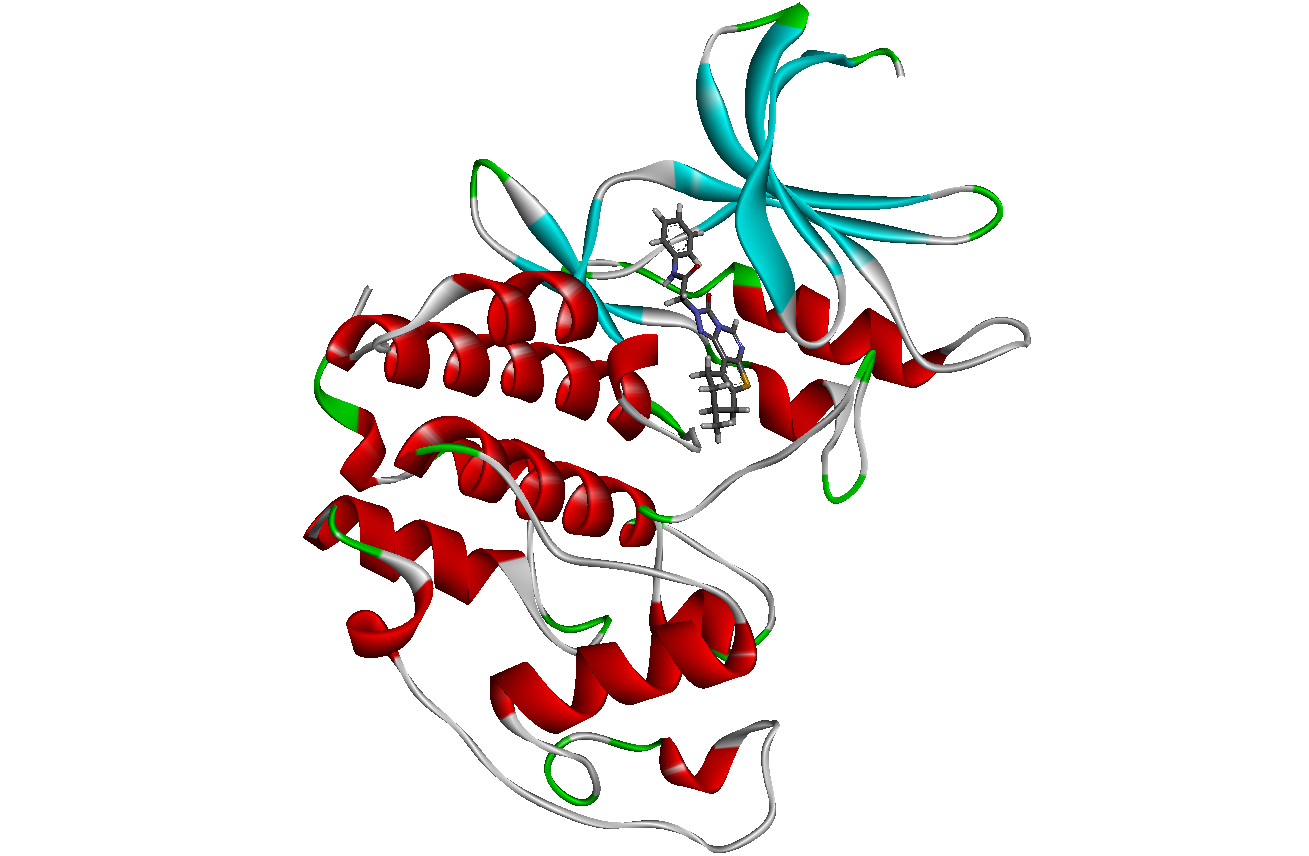
\includegraphics[width=\linewidth]{Case/CCRKHomologousModel.png}
\caption{CCRK homologous model, built by Dr. William Cheung based on the CDK2 template with PDB ID 1HCL \citep{1142} using SWISS-MODEL. The ligand denotes the Ser/Thr protein kinase active site.}
\label{Case:CCRKHomologousModel}
\end{figure}

\begin{figure*}
\centering
\subfloat[Our CCRK homologous model in complex of ZINC03830332, which forms 4 hydrogen bonds with LYS33, LYS129 and TYR169, and Pi-Cation interactions with LYS33 and LYS129.]
{
  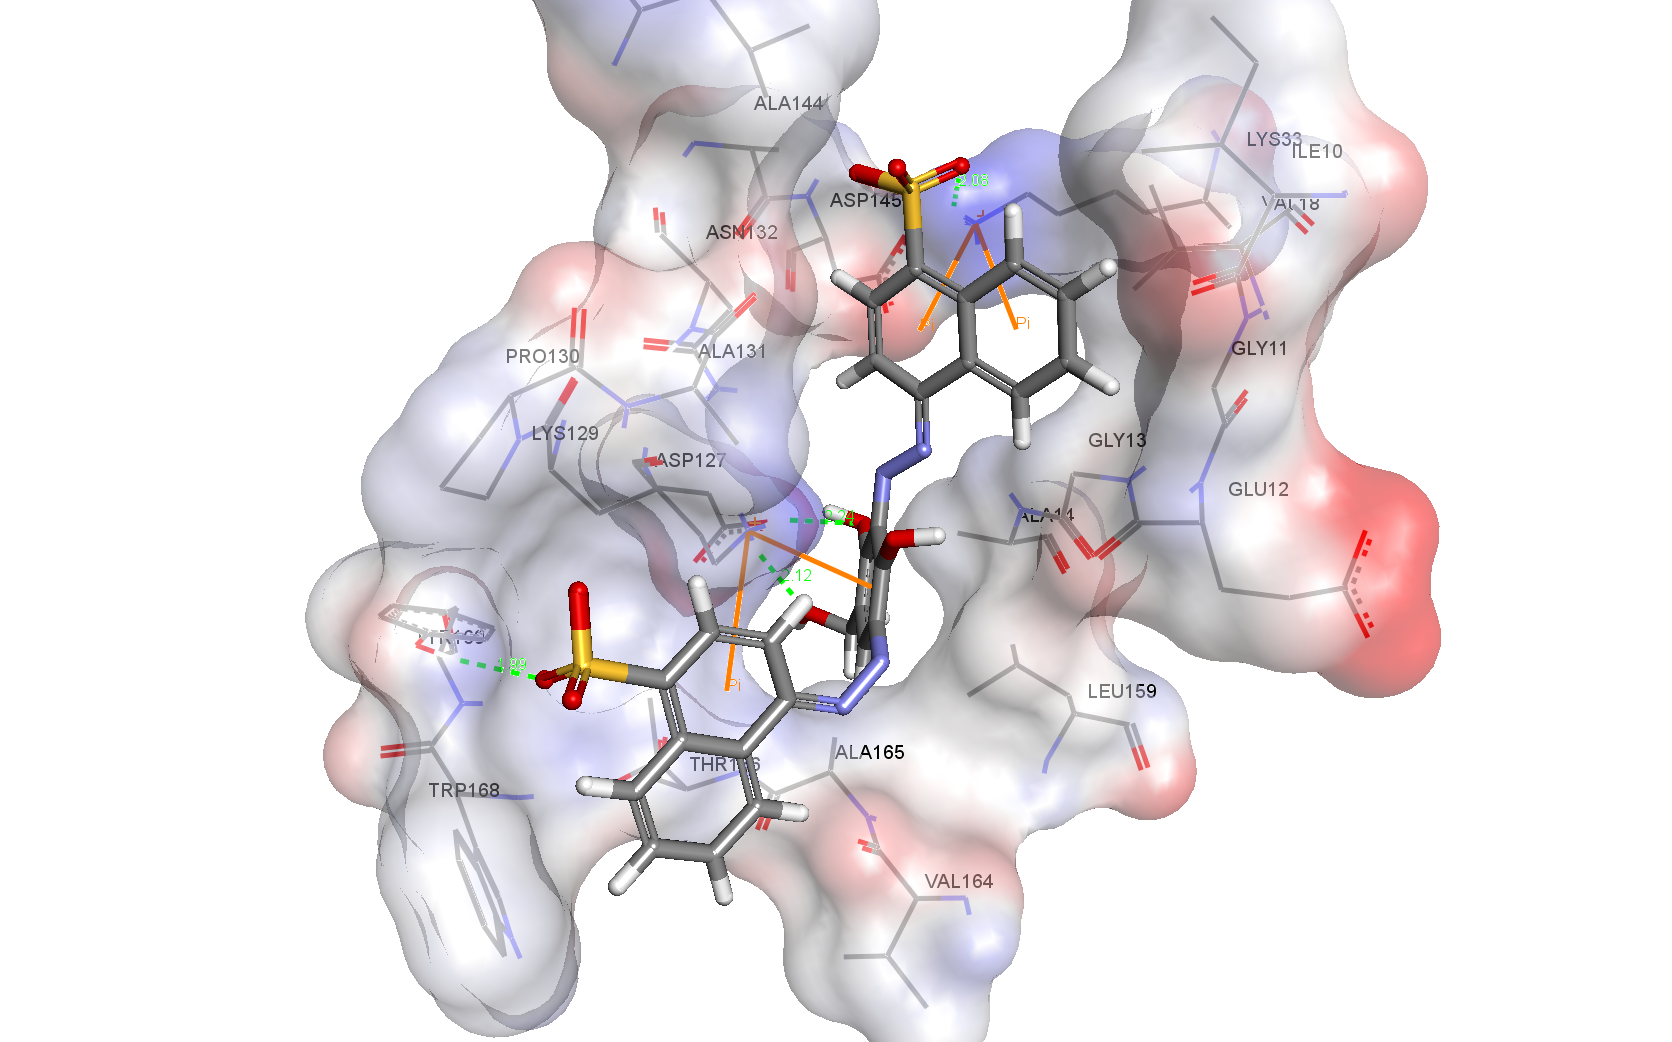
\includegraphics[width=0.485\linewidth]{Case/1HCL-ZINC03830332.png}
}
\subfloat[Our CCRK homologous model in complex of ZINC03831625, which forms 7 hydrogen bonds with HIS15, LYS33, LYS129, ASN132 and ASP145.]
{
  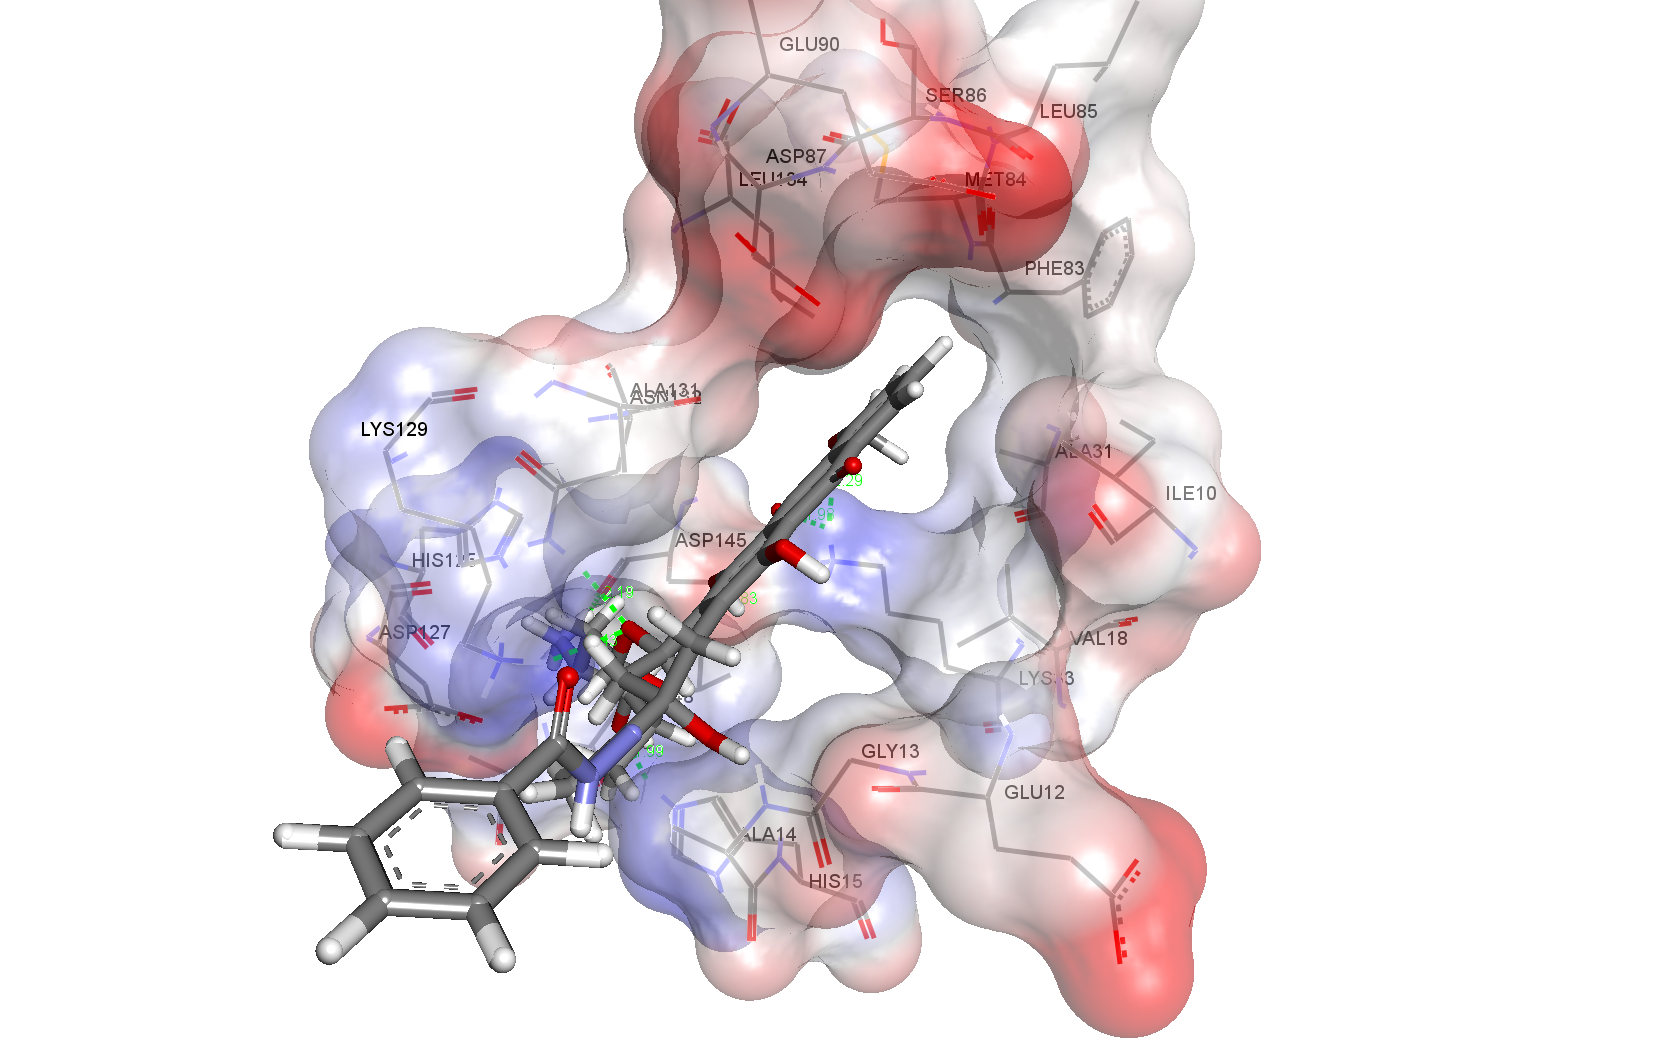
\includegraphics[width=0.485\linewidth]{Case/1HCL-ZINC03831625.png}
}
\caption{Two high-rank ligands for our CCRK homologous model.}
\label{Case:1HCLHits}
\end{figure*}

\bibliographystyle{unsrtnat}
\bibliography{../refworks}

\end{document}
